\chapter{From WPT to WIPT}
In this section, we first introduce a general WPT architecture. Next, we focus on the rectenna behavior and derive the analytical diode models for the energy harvester. We then extend the work to WIPT and explore two practical receiver structures. Finally, the signal and system model is established, and the dependency of delivered power on signal design is investigated on top of it.

\section{WPT Architecture}\label{sec:wpt-architecture}
  Figure {block_diagram} [book] presents the schematic diagram of a general WPT system. The operating principle can be classified into \textit{maximum power transfer} and \textit{maximum power efficiency transfer} [A Critical]. This article is based on the efficiency criterion to reach a compromise between the harvested power and the physical limitation. As suggested in [book], the overall power transmit efficiency $e$ can be decomposed as

\begin{equation}\label{eqn:power_utilization_efficiency}
  e = \frac{{{P_{{\text{dc}},{\text{ST}}}}}}{{P_{{\text{dc}}}^t}} = \underbrace {\frac{{P_{{\text{rf}}}^t}}{{P_{{\text{dc}}}^t}}}_{{e_1}} \cdot \underbrace {\frac{{P_{{\text{rf}}}^r}}{{P_{{\text{rf}}}^t}}}_{{e_2}} \cdot \underbrace {\frac{{P_{{\text{dc}}}^r}}{{P_{{\text{rf}}}^r}}}_{{e_3}} \cdot \underbrace {\frac{{{P_{{\text{dc}},{\text{ST}}}}}}{{P_{{\text{dc}}}^r}}}_{{e_4}}
\end{equation}

where the power transmitter determines the DC-to-RF efficiency ${e_1}$, the channel influences the RF-to-RF efficiency ${e_2}$, the rectenna decides the RF-to-DC efficiency ${e_3}$, and the power management unit (PMU) deals with the DC-to-DC efficiency ${e_4}$. Most existing solutions assume no dependency in between and focus on maximizing each term individually [see ref] then concatenate them together. Specifically, ${e_1}$ ${e_3}$ and ${e_4}$ are often neglected in waveform design and resource allocation. Interestingly, it has been proved by [Communications and][Waveform design][Practical nonlinear] that these efficiencies are coupled with each other, and the problem requires a joint optimization. Indeed, the RF-to-DC efficiency ${e_3}$ is observed to be a nonlinear function of the rectifier input power ${P_{{\text{rf}}}^r}$ [Towards the][Maximum achievable][Power-optimized], which also depends on signal waveform [Optimum waveform][Boosting the]. This article employs a tractable nonlinear harvester model proposed in [Waveform design] that was proved beneficial to the harvested current. 

\section{Rectenna Design}\label{sec:rectenna-design}
  \subsection{Rectenna Behavior}\label{sec:rectenna-behavior}

A rectenna receives electromagnetic power with antenna and convert it to electric power with rectifier. Diverse configurations are available for energy harvesting, such as \textit{Schottky} \cite{Akkermans2005, Boaventura2013}, \textit{CMOS} \cite{Stoopman2014, Valenta2014}, \textit{series} \cite{Georgiadis2011, Collado2013}, \textit{shunt} \cite{McSpadden1998, Guo2012}. Interestingly, those models are not equally suitable for the same input power, and maximizing the rectenna efficiency ${e_3}$ requires a proper selection according to the power range. As reported in \cite{Valenta2014, Costanzo2016}, low barrier Schottky diodes are commonly used for input power between \SI{1}{\uW} and \SI{1}{\mW}. Specifically, single diode is preferred for low power below \SI{500}{\uW} and multiple diodes are typically applied for input power above \SI{500}{\uW} \cite{Clerckx2019}. Hybrid designs as \cite{Sun2013} may be employed to maintain a high efficiency for large power range.

Besides the rectenna model, the shape of the received signal also influences the RF-to-DC efficiency ${e_3}$. It was first demonstrated in \cite{Trotter2009} that multisine waveform \textit{i.e. Power-Optimized waveform (POW)} outperforms the single tone waveform \textit{i.e. Continuous Wave (CW)} in operation range and power efficiency. The expression of a multisine waveform with $N$ subcarriers writes as a summation of $N$ sine waves:

\begin{equation}\label{eqn:multisine}
  {V_{{\text{multisine}}}}(t) = \sum\limits_{n = 0}^{N - 1} {\frac{1}{{\sqrt N }}} \sin \left( {2\pi \left( {{f_{\text{0}}} + n\Delta f} \right)t} \right)
\end{equation}

where ${{f_{\text{0}}}}$ is the minimum frequency and ${\Delta f}$ is the spacing. Figure \ref{fig:waveform_comparison} \cite{Trotter2009} illustrates the three-subcarrier case for both signals in time and frequency domains. It can be observed that multisine waveform provides a higher PAPR equals to ${\sqrt N }$ and occupies a bandwidth of $(N - 1) \Delta f$ with the same average power as CW, which is equally distributed to its components.

\begin{figure}
  \centering

  \begin{subfigure}{.45\textwidth}
    \centering
      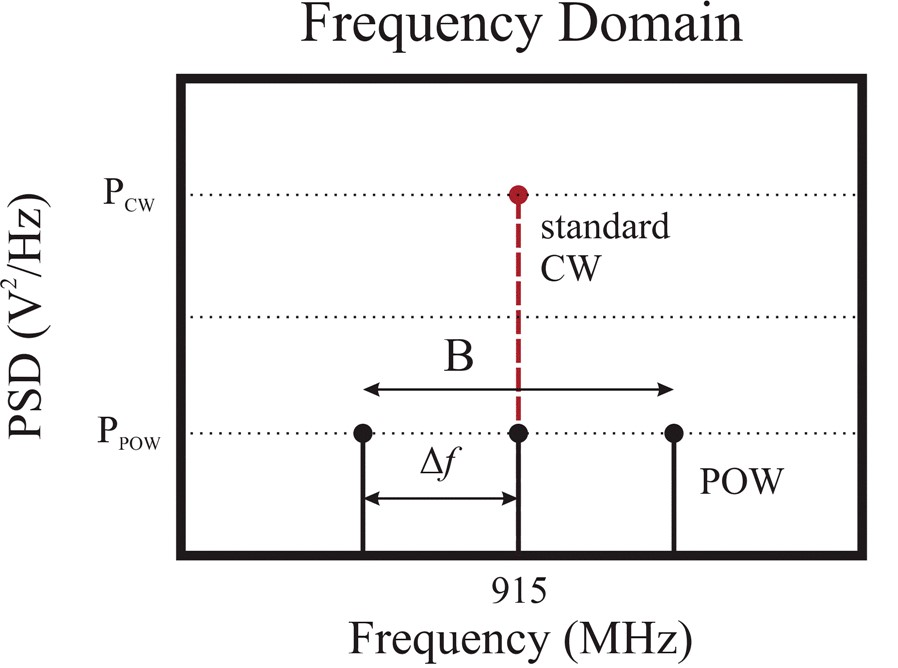
\includegraphics[width=\textwidth]{waveform_frequency_domain}
    \caption{Frequency domain}
    \label{fig:waveform_frequency_domain}
  \end{subfigure}
  \begin{subfigure}{.45\textwidth}
    \centering
      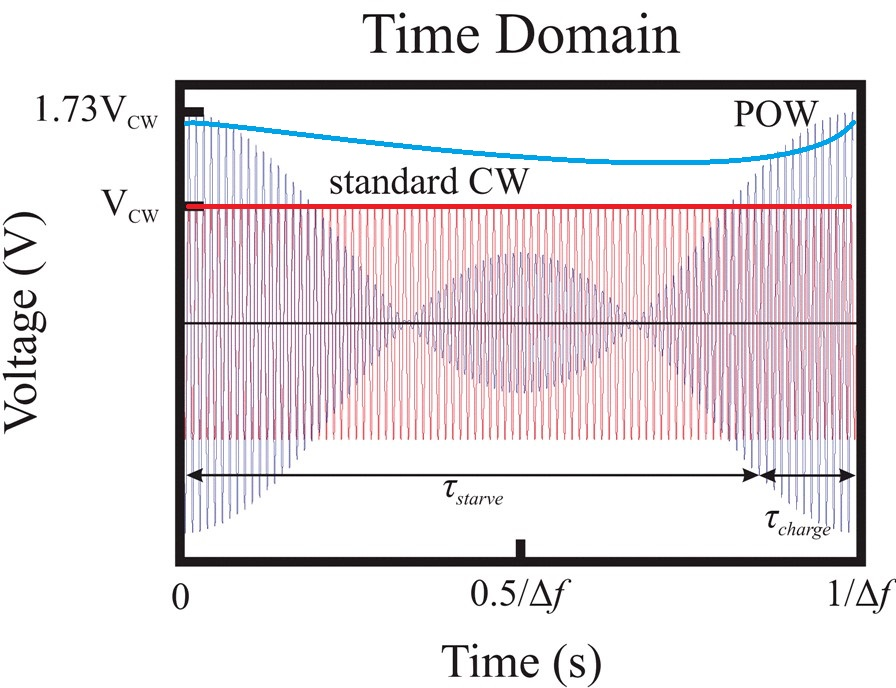
\includegraphics[width=\textwidth]{waveform_time_domain}
    \caption{Time domain}
    \label{fig:waveform_time_domain}
  \end{subfigure}

  \caption{Comparison of a typical 3-subcarrier multisine and CW in time and frequency domains (modified from \cite{Trotter2009}). The thick lines are examples of rectifier output voltage.}
  \label{fig:waveform_comparison}
\end{figure}

The advantage of multisine in WPT is that the high PAPR increases the peak rectifier output voltage. With a proper signal and circuit design, high voltage may be preserved during the cycle if discharging is slow enough, as indicated by the thick blue line in Figure \ref{fig:waveform_time_domain}. To enhance the harvested power, a large number of tones may be used to increase PAPR, and the multisine signal will appear as pulses with period of $1/\Delta f$. Most of the signal power will be concentrated in those pulses to trigger the diode and charge the capacitor. However, more subbands can lead to smaller frequency gaps and longer charging cycle when the bandwidth is fixed.

It can be hard to derive an accurate expression of the RF-to-DC efficiency ${e_3}$ on the power and shape of the rectifier input signal, as practical energy harvesting circuits consists of various nonlinear components as diodes, capacitors and inductors. It is also sensitive to parasitic sources, impedance matching, and harmonic generation \cite{Strassner2013, Valenta2014}. In this article, we employ the \textit{diode linear model} and \textit{diode nonlinear model} proposed in \cite{Clerckx2016} based on the diode current-voltage (I-V) characteristics to capture the fundamental pattern of rectenna and investigate its impact on resource allocation and system design. A superposed waveform containing modulated information and multisine power components is optimized according to CSI on top of both models.



\subsection{Antenna Model}\label{sec:antenna-model}

As illustrated by Figure \ref{fig:single_diode_rectifier}, the rectifier consists of a single diode as the source of nonlinearity and a low-pass filter to store energy.

\begin{figure}
  \centering

  \begin{subfigure}{.45\textwidth}
    \centering
      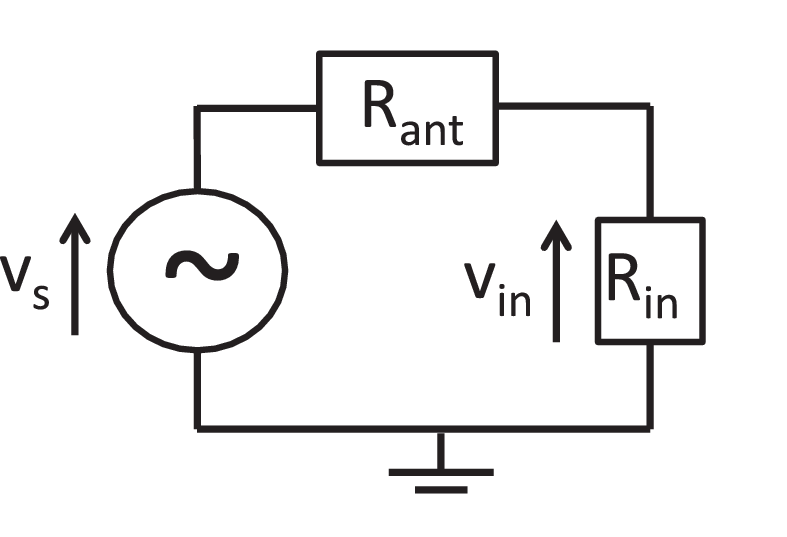
\includegraphics[width=\textwidth]{antenna_equivalent_circuit}
    \caption{Antenna equivalent circuit}
    \label{fig:antenna_equivalent_circuit}
  \end{subfigure}
  \begin{subfigure}{.45\textwidth}
    \centering
      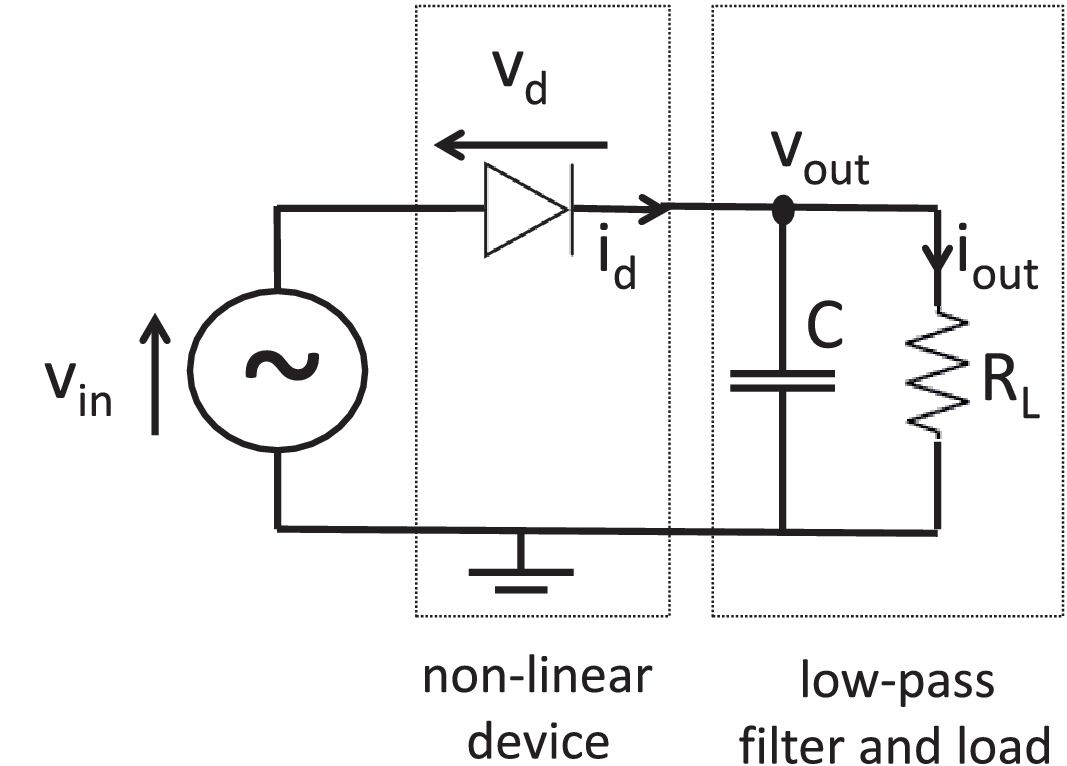
\includegraphics[width=\textwidth]{single_diode_rectifier}
    \caption{A single diode rectifier}
    \label{fig:single_diode_rectifier}
  \end{subfigure}

  \caption{Rectenna architecture}
  \label{fig:rectenna_architecture}
\end{figure}

Figure \ref{fig:antenna_equivalent_circuit} shows that the antenna equivalent circuit includes a voltage source ${v_{\text{s}}}(t)$ connected to a series antenna impedance ${Z_{{\text{ant}}}} = {R_{{\text{ant}}}} + j{X_{{\text{ant}}}}$ followed by a combined impedance of the rectifier and the matching network ${Z_{{\text{in}}}} = {R_{{\text{in}}}} + j{X_{{\text{in}}}}$. Assuming lossless, the perfect matching condition is

\begin{equation}\label{eqn:perfect_match}
  {R_{{\text{in}}}} = {R_{{\text{ant}}}},{X_{{\text{in}}}} =  - {X_{{\text{ant}}}}
\end{equation}

When equation \ref{eqn:perfect_match} is satisfied, the rectifier input voltage equals

\begin{equation}\label{eqn:rectifier_input_voltage}
  {v_{{\text{in}}}}(t) = {v_{\text{s}}}(t)/2 = y(t)\sqrt {{R_{{\text{in}}}}}
\end{equation}

where ${y(t)}$ is the received signal. Therefore, the input power to the rectifier writes

\begin{equation}\label{eqn:rectifier_input_power}
  P_{{\text{rf}}}^r = \mathbb{E}\left[ {y{{(t)}^2}} \right] = \mathbb{E}\left[ {{v_{{\text{in}}}}{{(t)}^2}} \right]/{R_{{\text{in}}}}
\end{equation}

It is also assumed that the noise is too small to be harvested.



\section{Receiver Architectures}\label{sec:receiver-architectures}
  We investigated two practical architectures for the co-located integrated information and energy receiver. Both designs are equipped with individual ID and EH receivers. The former is a conventional baseband demodulator while the latter can be implemented with the proposed rectifier structure in Section \ref{sec:rectenna-design}.



\subsection{Time Switching}\label{sec:time-switching}
A \textit{Time Switching} (TS) receiver (Fig. \ref{fig:ts-receiver}) operates as either an information decoder or an energy harvester at a fixed time. In the design, the transmitter divides the transmission block into orthogonal power and data slots with length ratios $\alpha $ and $1 - \alpha $ respectively. It then optimizes the waveform for WPT or WIT individually. On the other hand, the receiver periodically switches between ID and EH receivers in the corresponding slots. Perfect synchronization between transmitter and receiver is required for precise mode control. It can achieve different rate-energy tradeoffs by adjusting the slot length ratio $\alpha $ jointly with the transmit signals. Since the information decoder and energy harvester may work in different power ranges, TS can be combined with a "near-far" scheduling \cite{Zhang2013} to benefit the system efficiency.

\begin{figure}[ht]
  \centering
    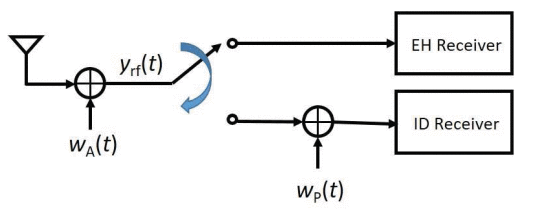
\includegraphics[width=\textwidth]{ts_receiver}
  \caption{Structure of TS receiver \cite{Clerckx2019}}
  \label{fig:ts-receiver}
\end{figure}



\subsection{Power Splitting}\label{sec:power-splitting}
In \textit{Power Splitting} (PS) receiver (Fig. \ref{fig:ps-receiver}), we introduce a PS ratio $\rho $ to split the received signal into individual power stream (with proportion $\rho $) and information stream (with proportion $1 - \rho $). At the transmitter, the signal is jointly optimized for information and power transmission according to CSIT. When perfectly matched, the EH and ID receivers are with input voltage $\sqrt {\rho {R_{{\text{ant}}}}} y(t)$ and $\sqrt {(1 - \rho ){R_{{\text{ant}}}}} y(t)$ respectively. Different rate-energy pairs can be obtained by varying the PS ratio $\rho $. It is argued in \cite{Zhang2013} that PS is the best strategy for linear harvester model with negligible RF-to-baseband noise, but \cite{Clerckx2016} demonstrated that the PS-only transmission is suboptimal when considering rectifier nonlinearity.

\begin{figure}[ht]
  \centering
    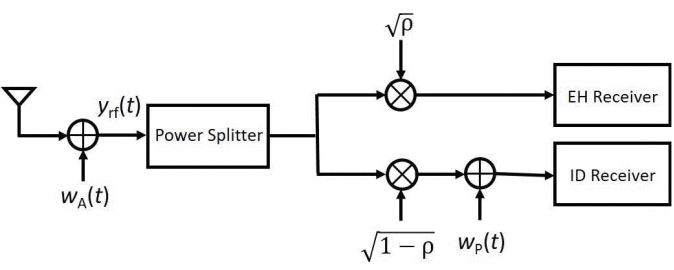
\includegraphics[width=0.8\textwidth]{ps_receiver}
  \caption{Structure of PS receiver \cite{Clerckx2019}}
  \label{fig:ps-receiver}
\end{figure} 

\section{Signal and System Model}\label{sec:signal-and-system-model}
  Consider a point-to-point MISO WIPT system in multipath environment. The $M$-antenna transmitter delivers information and power simultaneously to the single-antenna receiver through $N$ orthogonal subbands. It is assumed the carrier frequencies are with even spacing $\Delta f$ and equal bandwidth ${B_{\text{s}}}$. The $n$-th subband has carrier frequency ${f_n} = {f_0} + n\Delta f$ for $n = 0, \ldots ,N - 1$. To maximize the rate-energy tradeoff, we employ a superposed signal consists of a multi-carrier deterministic multisine waveform and a multi-carrier random modulated waveform for WIPT. Both components are transmitted on the same frequency bands.



\subsection{Transmitted Information Waveform}\label{sec:transmitted-information-waveform}
Denote the information symbol carried by the modulated waveform on subband $n$ as ${{\tilde x}_n}$, we assume the input symbol is with the capacity-achieving i.i.d. Circular Symmetric Complex Gaussian (CSCG) distribution with zero mean and unit variance \cite{Varasteh2017a}:

\begin{equation}\label{eqn:unmodulated_symbol}
  {{\tilde x}_n} = \left| {{{\tilde x}_n}} \right|{e^{j{\phi _{{{\tilde x}_n}}}}}\sim\mathcal{C}\mathcal{N}(0,1)
\end{equation}

Hence, the modulated waveform on antenna $m = 1, \ldots ,M$, subband $n$ writes as

\begin{equation}\label{eqn:modulated_symbol}
  {x_{n,m}} = {w_{I,n,m}}{{\tilde x}_n}
\end{equation}

where ${w_{I,n,m}}$ is the corresponding information weight and is a constant for a certain channel state:

\begin{equation}\label{eqn:weight_information}
  {w_{I,n,m}} = \left| {{w_{I,n,m}}} \right|{e^{j{\phi _{I,n,m}}}} = {s_{I,n,m}}{e^{j{\phi _{I,n,m}}}}
\end{equation}

Note the amplitude and phase are separated in resource allocation. Define matrices ${{\mathbf{S}}_I}$ and ${{\mathbf{\Phi }}_I}$ of size $N \times M$ such that the $(n,m)$ entries hold ${s_{I,n,m}}$ and ${\phi _{I,n,m}}$ respectively, the design of information waveform is converted into an optimization problem on both matrices, with the average WIT transmit power ${P_I} = \frac{1}{2}\left\| {{{\mathbf{S}}_I}} \right\|_F^2$. The modulated symbol of equation \ref{eqn:modulated_symbol} can be further expressed as

\begin{equation}\label{eqn:modulated_symbol_further}
  {x_{n,m}} = {s_{I,n,m}}{e^{j{\phi _{I,n,m}}}} \cdot \left| {{{\tilde x}_n}} \right|{e^{j{\phi _{{{\tilde x}_n}}}}} = {{\tilde s}_{I,n,m}}{e^{j{{\tilde \phi }_{I,n,m}}}}
\end{equation}

with ${{\tilde s}_{I,n,m}} = {s_{I,n,m}}\left| {{{\tilde x}_n}} \right|$ and ${{\tilde \phi }_{I,n,m}} = {\phi _{I,n,m}} + {\phi _{{{\tilde x}_n}}}$. In this way, the impact of symbol distribution and waveform design are combined. The modulated waveform also follows an i.i.d. CSCG distribution with variance equal to the subband power ${x_{n,m}}\sim\mathcal{C}\mathcal{N}\left( {0,s_{I,n,m}^2} \right)$.

Therefore, the information waveform ${x_{I,m}}(t)$ on antenna $m$ at time $t$ writes as

\begin{align}\label{eqn:information_waveform}
  {x_{I,m}}(t) &= \sum\limits_{n = 0}^{N - 1} {{{\tilde s}_{I,n,m}}(t)\cos \left( {2\pi {f_n}t + {{\tilde \phi }_{I,n,m}}(t)} \right)}  \hfill \\
   &= \Re \left\{ {\sum\limits_{n = 0}^{N - 1} {{x_{n,m}}(t){e^{j2\pi {f_n}t}}} } \right\} \hfill \\
   &= \Re \left\{ {\sum\limits_{n = 0}^{N - 1} {{w_{I,n,m}}{{\tilde x}_n}(t){e^{j2\pi {f_n}t}}} } \right\} \hfill
\end{align}

On top of this, the WIT signal vector is spread over $M$ antennas

\begin{equation}\label{eqn:wit_vector}
  {{\mathbf{x}}_I}(t) = \Re \left\{ {\sum\limits_{n = 0}^{N - 1} {{{\mathbf{w}}_{I,n}}} {{\tilde x}_n}(t){e^{j2\pi {f_n}t}}} \right\}
\end{equation}

where ${{\mathbf{w}}_{I,n}} = {\left[ {{w_{I,n,1}} \cdots {w_{I,n,M}}} \right]^T}$.



\subsection{Transmitted Power Waveform}\label{sec:transmitted-power-waveform}
Comparing with the information component, the multisine power component is unmodulated and deterministic, so there is no dependency on the distribution of input symbol $\tilde{x}_{n}(t)$. The power waveform on antenna $m$, subband $n$ is given by

\begin{equation}\label{eqn:unmodulated}
  {w_{P,n,m}} = {s_{P,n,m}}{e^{j{\phi _{P,n,m}}}}
\end{equation}

where ${s_{P,n,m}}$ and ${{\phi _{P,n,m}}}$ are the amplitude and phase of the multisine signal. Collect them into the $(n,m)$ entries of matrices ${{\mathbf{S}}_P}$ and ${{\mathbf{\Phi }}_P}$, the average power of the WPT waveform is $\frac{1}{2}\left\|\mathbf{S}_{P}\right\|_{F}^{2}$. Similarly, the power waveform ${x_{P,m}}(t)$ on antenna $m$ at time $t$ is

\begin{align}\label{eqn:power_waveform}
  {x_{P,m}}(t) &= \sum\limits_{n = 0}^{N - 1} {{s_{P,n,m}}\cos \left( {2\pi {f_n}t + {\phi _{P,n,m}}} \right)}  \hfill \\
   &= \Re \left\{ {\sum\limits_{n = 0}^{N - 1} {{w_{P,n,m}}{e^{j2\pi {f_n}t}}} } \right\} \hfill
\end{align}

Combine the power signals on all $M$ antennas, the WPT signal vector writes as

\begin{equation}\label{eqn:wpt_vector}
  {{\mathbf{x}}_P}(t) = \Re \left\{ {\sum\limits_{n = 0}^{N - 1} {{{\mathbf{w}}_{P,n}}} {e^{j2\pi {f_n}t}}} \right\}
\end{equation}

with ${{\mathbf{w}}_{P,n}} = {\left[ {{w_{P,n,1}} \cdots {w_{P,n,M}}} \right]^T}$.



\subsection{Multipath Channel and Received Signal}\label{sec:multipath-and-received-signal}
Consider a multipath channel with $L$ paths. For the $l$-th path ($l = 1, \ldots ,L$), denote the phase shift between the receive antenna and transmit antenna $m$ of subband $n$ as ${\zeta _{n,m,l}}$. Let ${\tau _l}$ and ${\alpha _l}$ be the delay and magnitude gain, and indicate the transmit signal on subband $n$ of antenna $m$ as

\begin{equation}\label{eqn:superposed_waveform}
  {v_{n,m}}(t) = {w_{P,n,m}} + {w_{I,n,m}}{{\tilde x}_n}(t)
\end{equation}

The superposed signal containing modulated information waveform and multisine power waveform is demonstrated to bring a two-fold benefit on rate and energy \cite{Clerckx2019}. Also, the channel frequency response is expressed as

\begin{equation}\label{eqn:channel}
  {h_{n,m}} = \sum\limits_{l = 0}^{L - 1} {{\alpha _l}{e^{j\left( { - 2\pi {f_n}{\tau _l} + {\zeta _{n,m,l}}} \right)}}}  = {A_{n,m}}{e^{j{{\bar \psi }_{n,m}}}}
\end{equation}

To ensure $v_{n, m}(t)$ and $\tilde{x}_{n}(t)$ being narrowband signals, we assume ${\max _{l \ne {l^\prime }}}\left| {{\tau _l} - {\tau _{{l^\prime }}}} \right| <  < 1/{B_{\text{s}}}$. It is also supposed that ${v_{n,m}}\left( {t - {\tau _l}} \right) = {v_{n,m}}(t)$ and ${{\tilde x}_n}\left( {t - {\tau _l}} \right) = {{\tilde x}_n}(t)$. The received signal corresponding to transmit antenna $m$ contains the power component $y_{P, m}(t)$ and the information component $y_{I, m}(t)$

\begin{align}\label{eqn:received_signal_component}
  {y_m}(t) &= {y_{P,m}}(t) + {y_{I,m}}(t) \hfill \\
   &= \Re \left\{ {\sum\limits_{l = 0}^{L - 1} {\sum\limits_{n = 0}^{N - 1} {{\alpha _l}} } {v_{n,m}}\left( {t - {\tau _l}} \right){e^{j2\pi {f_n}\left( {t - {\tau _l}} \right) + {\zeta _{n,m,l}}}}} \right\} \hfill \\
   &\approx \Re \left\{ {\sum\limits_{n = 0}^{N - 1} {{h_{n,m}}} {v_{n,m}}(t){e^{j2\pi {f_n}t}}} \right\} \hfill
\end{align}

Hence, the total received signal can be obtained by stacking up equation \ref{eqn:received_signal_component} over all transmit signals

\begin{align}\label{eqn:received_signal}
  y(t) &= {y_P}(t) + {y_I}(t) \hfill \\
   &= \Re \left\{ {\sum\limits_{n = 0}^{N - 1} {{{\mathbf{h}}_n}} \left( {{{\mathbf{w}}_{P,n}} + {{\mathbf{w}}_{I,n}}{{\tilde x}_n}} \right){e^{j2\pi {f_n}t}}} \right\} \hfill
\end{align}

where the channel vector is defined as ${{\mathbf{h}}_n} = \left[ {{h_{n,1}} \ldots {h_{n,M}}} \right]$.  